%% Architecture diagrams for the final report, one per page.
%% Drawn from the architecture deck of 18 November 2026
%% (docs/report/insights/update_181126/s1_system.tex, s2_orb.tex, s3_vins.tex,
%% s4_rtab.tex); keep the two in step. Build: pdflatex architecture.tex
\documentclass[tikz,border=4pt]{standalone}
\usepackage[T1]{fontenc}
\usepackage{helvet}
\renewcommand{\familydefault}{\sfdefault}
\usepackage{amssymb}
\usepackage{xcolor}
\usetikzlibrary{arrows.meta,positioning,fit,calc,backgrounds,
                decorations.pathreplacing,shapes.geometric,shadows}
\newcommand{\repo}[1]{\texttt{\detokenize{#1}}}
\definecolor{sensorcol}{HTML}{2FB5E8}
\definecolor{perccol}{HTML}{26A69A}
\definecolor{plancol}{HTML}{F2735A}
\definecolor{ctrlcol}{HTML}{8FA3BA}
\definecolor{mapcol}{HTML}{34495E}
\definecolor{orbc}{HTML}{D6336C}
\definecolor{vinsc}{HTML}{E67E22}
\definecolor{rtabc}{HTML}{27AE60}
\definecolor{navc}{HTML}{2E86DE}
\definecolor{sysc}{HTML}{5D6D7E}
\definecolor{dimg}{HTML}{E74C3C}
\definecolor{dimu}{HTML}{F39C12}
\definecolor{dwhl}{HTML}{16A085}
\definecolor{dpose}{HTML}{8E44AD}
\definecolor{dmap}{HTML}{2C3E50}
\definecolor{dcmd}{HTML}{2E86DE}
\definecolor{ourc}{HTML}{E0A100}
\definecolor{hlc}{HTML}{C0392B}
\definecolor{offc}{HTML}{AAB7B8}
\definecolor{good}{HTML}{1E8449}
\definecolor{bad}{HTML}{C0392B}
% ---------------------------------------------------------------- tikz styles
\tikzset{
  box/.style={draw=black!45, rounded corners=2pt, align=center, font=\scriptsize,
              inner sep=2pt, minimum height=8mm, text width=22mm, fill=white},
  arr/.style={-{Latex[length=1.8mm]}, thick, black!65},
  darr/.style={arr, dashed},
  rate/.style={font=\tiny, fill=white, inner sep=1pt, text=black!75, align=center},
  % "added by this project" and "switched off"
  ours/.style={draw=ourc, dashed, line width=1.2pt},
  off/.style={draw=offc, dashed, fill=offc!15, text=black!45},
  % the current component
  hl/.style={draw=hlc, line width=1.6pt, fill=yellow!35},
  % locator chips
  chip/.style={draw=black!35, rounded corners=1.5pt, align=center, font=\scriptsize,
               inner sep=1.5pt, minimum height=8mm, text width=17mm},
  grouplbl/.style={font=\scriptsize\bfseries, text=black!60},
  brace/.style={decorate, decoration={brace, amplitude=3pt, raise=2pt}, thick, black!40},
  % small drawing helpers for the stage panels
  pt/.style={circle, fill=#1, inner sep=0pt, minimum size=1.6mm},
  pt/.default=black,
  cam/.style={isosceles triangle, shape border rotate=#1, draw=black!70, fill=white,
              minimum width=4mm, minimum height=4mm, inner sep=0pt},
  cam/.default=0,
}
% Every component has a style of its own name, empty by default.
% \hl{ORB3} inside a frame turns that one component yellow-and-red, so the
% locator strip and the block diagram both show "you are here".
\tikzset{ORB1/.style={},ORB2/.style={},ORB3/.style={},ORB4/.style={},
         ORB5/.style={},ORB6/.style={},ORB7/.style={},ORB8/.style={},
         VINS1/.style={},VINS2/.style={},VINS3/.style={},VINS4/.style={},
         VINS5/.style={},VINS6/.style={},VINS7/.style={},
         RTAB1/.style={},RTAB2/.style={},RTAB3/.style={},RTAB4/.style={},
         RTAB5/.style={},RTAB6/.style={},RTAB7/.style={},RTAB8/.style={},RTAB9/.style={},
         NAV1/.style={},NAV2/.style={},NAV3/.style={},NAV4/.style={},
         NAV5/.style={},NAV6/.style={},NAV7/.style={},NAV8/.style={}}
\newcommand{\hl}[1]{\tikzset{#1/.style={hl}}}


\newcommand{\lane}[4]{%
  \node[anchor=east, align=right] at (-0.02,#1) {#2};
  \draw[black!15] (0,#1) -- (1,#1);
  \foreach \k in {1,...,#3} \draw[#4, line width=0.7pt]
    ({(\k-0.5)/#3},#1-0.18) -- ({(\k-0.5)/#3},#1+0.18);}


\begin{document}
%% page 1: the whole system
  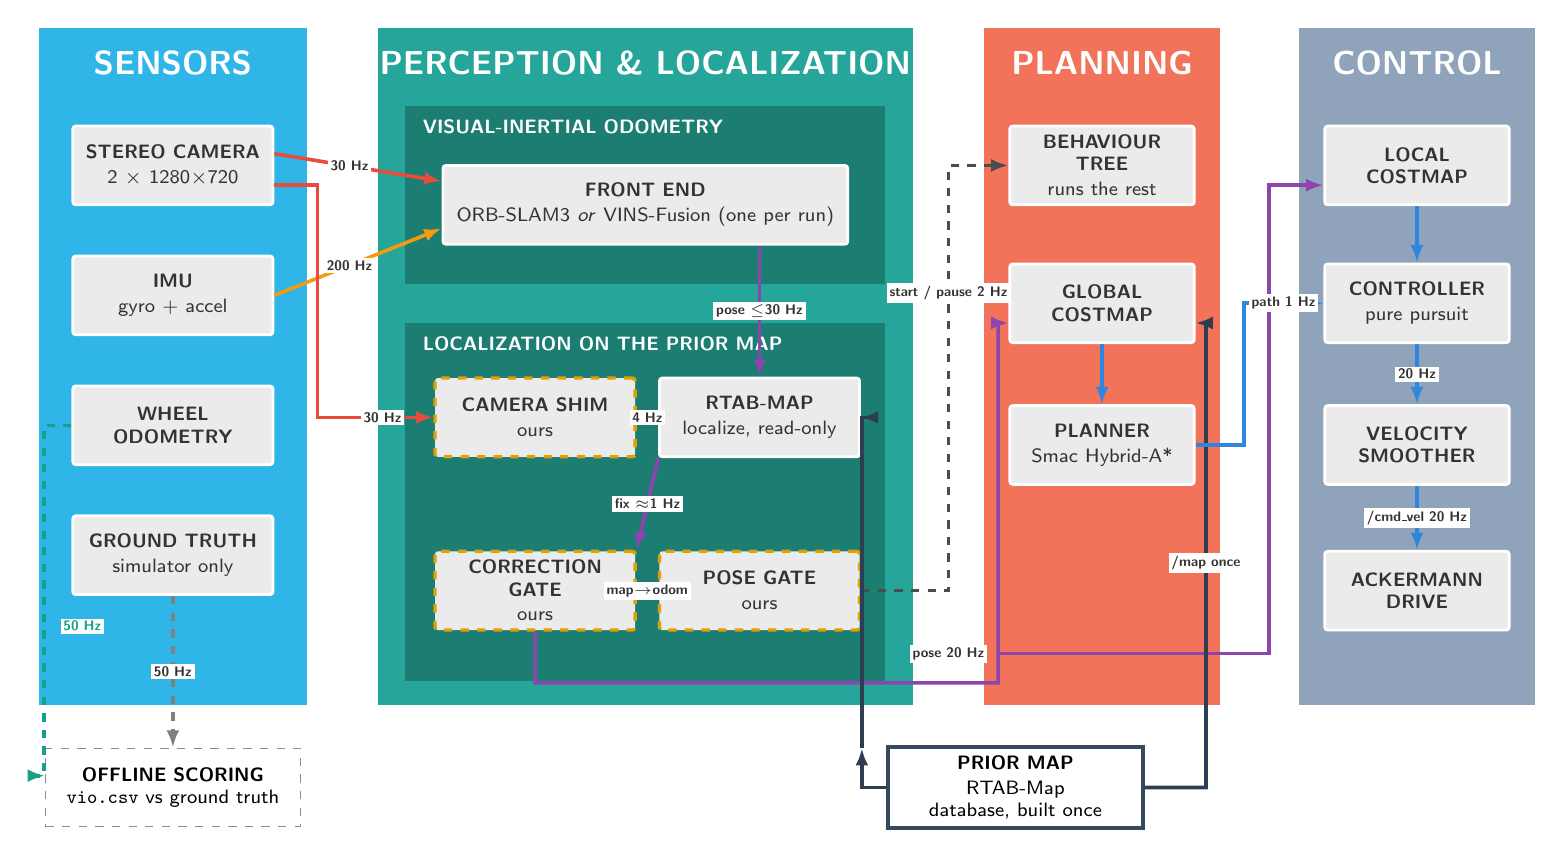
\begin{tikzpicture}[font=\footnotesize,
      ib/.style={draw=white, line width=1pt, rounded corners=1pt, align=center,
                 font=\scriptsize\bfseries, text=black!80, fill=white!92!black,
                 text width=24mm, minimum height=10mm, inner sep=2pt},
      hdr/.style={font=\large\bfseries, text=white},
      dl/.style={-{Latex[length=2.2mm]}, line width=1.3pt},
      rt/.style={font=\tiny\bfseries, fill=white, inner sep=1pt, text=black!80}]
    % ---------------- column panels
    \fill[sensorcol] (0,-4.4) rectangle (3.4,4.2);
    \node[hdr] at (1.7,3.75) {SENSORS};
    \fill[perccol] (4.3,-4.4) rectangle (11.1,4.2);
    \node[hdr] at (7.7,3.75) {PERCEPTION \& LOCALIZATION};
    \fill[plancol] (12.0,-4.4) rectangle (15.0,4.2);
    \node[hdr] at (13.5,3.75) {PLANNING};
    \fill[ctrlcol] (16.0,-4.4) rectangle (19.0,4.2);
    \node[hdr] at (17.5,3.75) {CONTROL};
    % sub-panels inside perception
    \fill[black!25!perccol] (4.65,0.95) rectangle (10.75,3.2);
    \node[font=\scriptsize\bfseries, text=white, anchor=north west] at (4.75,3.15)
      {VISUAL-INERTIAL ODOMETRY};
    \fill[black!25!perccol] (4.65,-4.1) rectangle (10.75,0.45);
    \node[font=\scriptsize\bfseries, text=white, anchor=north west] at (4.75,0.4)
      {LOCALIZATION ON THE PRIOR MAP};
    % ---------------- boxes
    \node[ib] at (1.7, 2.45) (cam) {STEREO CAMERA\\[1pt]\mdseries 2 $\times$ 1280$\times$720};
    \node[ib] at (1.7, 0.80) (imu) {IMU\\[1pt]\mdseries gyro + accel};
    \node[ib] at (1.7,-0.85) (whl) {WHEEL ODOMETRY};
    \node[ib] at (1.7,-2.50) (gt)  {GROUND TRUTH\\[1pt]\mdseries simulator only};
    \node[ib, text width=50mm] at (7.7, 1.95) (fe)
      {FRONT END\\[1pt]\mdseries ORB-SLAM3 \emph{or} VINS-Fusion (one per run)};
    \node[ib, ours] at (6.3,-0.75) (shim) {CAMERA SHIM\\[1pt]\mdseries ours};
    \node[ib]       at (9.15,-0.75) (rtab) {RTAB-MAP\\[1pt]\mdseries localize, read-only};
    \node[ib, ours] at (6.3,-2.95) (cg) {CORRECTION GATE\\[1pt]\mdseries ours};
    \node[ib, ours] at (9.15,-2.95) (pg) {POSE GATE\\[1pt]\mdseries ours};
    \node[ib, text width=22mm] at (13.5, 2.45) (bt)  {BEHAVIOUR TREE\\[1pt]\mdseries runs the rest};
    \node[ib, text width=22mm] at (13.5, 0.70) (gcm) {GLOBAL COSTMAP};
    \node[ib, text width=22mm] at (13.5,-1.10) (pl)  {PLANNER\\[1pt]\mdseries Smac Hybrid-A*};
    \node[ib, text width=22mm] at (17.5, 2.45) (lcm) {LOCAL COSTMAP};
    \node[ib, text width=22mm] at (17.5, 0.70) (ct)  {CONTROLLER\\[1pt]\mdseries pure pursuit};
    \node[ib, text width=22mm] at (17.5,-1.10) (sm)  {VELOCITY\\SMOOTHER};
    \node[ib, text width=22mm] at (17.5,-2.95) (drv) {ACKERMANN\\DRIVE};
    % MAP and SCORING, under the panels as in the reference
    \node[draw=mapcol, line width=1.3pt, fill=white, font=\scriptsize\bfseries,
          align=center, text width=30mm, minimum height=10mm] at (12.4,-5.45) (map)
      {PRIOR MAP\\[1pt]\mdseries RTAB-Map database, built once};
    \node[draw=black!45, dashed, fill=white, font=\scriptsize, align=center,
          text width=30mm, minimum height=10mm] at (1.7,-5.45) (eval)
      {\textbf{OFFLINE SCORING}\\ \repo{vio.csv} vs ground truth};
    % ---------------- data lines (colour = kind of data)
    \draw[dl, dimg] ($(cam.east)+(0,0.15)$) -- node[rt, pos=0.45]{30 Hz} ($(fe.west)+(0,0.30)$);
    \draw[dl, dimu] (imu.east) -- node[rt, pos=0.45]{200 Hz} ($(fe.west)+(0,-0.30)$);
    \draw[dl, dimg] ($(cam.east)+(0,-0.25)$) -- ++(0.55,0) |- node[rt, pos=0.78]{30 Hz} (shim.west);
    \draw[dl, dimg] (shim.east) -- node[rt]{4 Hz} (rtab.west);
    \draw[dl, dpose] (fe.south -| rtab.north) -- node[rt]{pose $\le$30 Hz} (rtab.north);
    \draw[dl, dpose] (rtab.south west) -- node[rt, pos=0.5]{fix $\approx$1 Hz} (cg.north east);
    \draw[dl, dpose] (cg.east) -- node[rt]{map$\rightarrow$odom} (pg.west);
    % the robot's pose reaches planning and control through TF
    \draw[dl, dpose] (cg.south) -- ++(0,-0.65) -| (12.18,0.45) -- ($(gcm.west)+(0,-0.25)$);
    \draw[dl, dpose] (12.18,-3.75) -| (15.62,2.2) -- ($(lcm.west)+(0,-0.25)$);
    \node[rt] at (11.55,-3.75) {pose 20 Hz};
    % gate decides whether Nav2 runs at all
    \draw[dl, black!70, dashed] (pg.east) -- (11.55,-2.95) |- node[rt, pos=0.35]{start / pause 2 Hz} (bt.west);
    % the map
    \draw[dl, dmap] (10.45,-4.95) |- (rtab.east);
    \draw[dl, dmap] (map.west) -- (10.45,-5.45) -- (10.45,-4.95);
    \draw[dl, dmap] (map.east) -| (14.82,0.45) -- ($(gcm.east)+(0,-0.25)$);
    \node[rt] at (14.82,-2.6) {/map once};
    % planning -> control
    \draw[dl, dcmd] (gcm) -- (pl);
    \draw[dl, dcmd] (pl.east) -- (15.3,-1.10) |- node[rt, pos=0.75]{path 1 Hz} (ct.west);
    \draw[dl, dcmd] (lcm) -- (ct);
    \draw[dl, dcmd] (ct) -- node[rt]{20 Hz} (sm);
    \draw[dl, dcmd] (sm) -- node[rt]{/cmd\_vel 20 Hz} (drv);
    % offline
    \draw[dl, dwhl, dashed] (whl.west) -- ++(-0.35,0) |- ($(eval.west)+(0,0.15)$);
    \draw[dl, black!50, dashed] (gt.south) -- node[rt]{50 Hz} (eval.north);
    \node[rt, text=dwhl] at (0.55,-3.4) {50 Hz};
  \end{tikzpicture}
%% page 2: ORB-SLAM3
  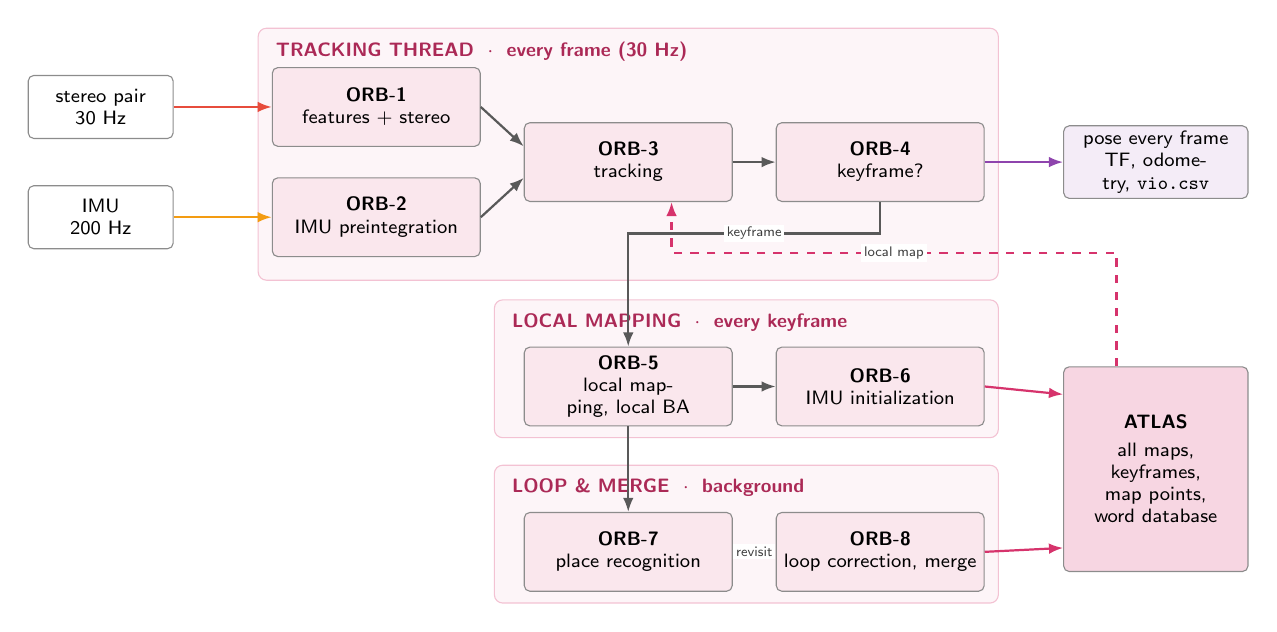
\begin{tikzpicture}[font=\scriptsize,
      cb/.style={box, fill=orbc!12, text width=25mm, minimum height=10mm},
      band/.style={fill=orbc!5, draw=orbc!30, rounded corners=3pt},
      bl/.style={font=\scriptsize\bfseries, text=orbc!80!black, anchor=north west}]
    % thread bands
    \fill[band] (2.0,-1.75) rectangle (11.4,1.45);
    \node[bl] at (2.1,1.4) {TRACKING THREAD \;$\cdot$\; every frame (30 Hz)};
    \fill[band] (5.0,-3.75) rectangle (11.4,-2.0);
    \node[bl] at (5.1,-2.05) {LOCAL MAPPING \;$\cdot$\; every keyframe};
    \fill[band] (5.0,-5.85) rectangle (11.4,-4.1);
    \node[bl] at (5.1,-4.15) {LOOP \& MERGE \;$\cdot$\; background};
    % inputs
    \node[box, text width=17mm] (st) at (0,0.45) {stereo pair\\30 Hz};
    \node[box, text width=17mm] (im) at (0,-0.95) {IMU\\200 Hz};
    % components
    \node[cb, ORB1] (o1) at (3.5,0.45)  {\textbf{ORB-1}\\features + stereo};
    \node[cb, ORB2] (o2) at (3.5,-0.95) {\textbf{ORB-2}\\IMU preintegration};
    \node[cb, ORB3] (o3) at (6.7,-0.25) {\textbf{ORB-3}\\tracking};
    \node[cb, ORB4] (o4) at (9.9,-0.25) {\textbf{ORB-4}\\keyframe?};
    \node[cb, ORB5] (o5) at (6.7,-3.1)  {\textbf{ORB-5}\\local mapping, local BA};
    \node[cb, ORB6] (o6) at (9.9,-3.1)  {\textbf{ORB-6}\\IMU initialization};
    \node[cb, ORB7] (o7) at (6.7,-5.2)  {\textbf{ORB-7}\\place recognition};
    \node[cb, ORB8] (o8) at (9.9,-5.2)  {\textbf{ORB-8}\\loop correction, merge};
    % outputs and the map store
    \node[box, text width=22mm, fill=dpose!10] (out) at (13.4,-0.25)
      {pose every frame\\TF, odometry, \repo{vio.csv}};
    \node[box, text width=22mm, minimum height=26mm, fill=orbc!20] (atl) at (13.4,-4.15)
      {\textbf{ATLAS}\\[2pt]all maps,\\keyframes,\\map points,\\word database};
    % flow
    \draw[arr, dimg] (st) -- (o1);
    \draw[arr, dimu] (im) -- (o2);
    \draw[arr] (o1.east) -- ($(o3.west)+(0,0.2)$);
    \draw[arr] (o2.east) -- ($(o3.west)+(0,-0.2)$);
    \draw[arr] (o3) -- (o4);
    \draw[arr, dpose] (o4.east) -- (out.west);
    \draw[arr] (o4.south) -- ++(0,-0.4) -| node[rate, pos=0.25]{keyframe} (o5.north);
    \draw[arr] (o5) -- (o6);
    \draw[arr] (o5) -- (o7);
    \draw[arr] (o7) -- node[rate]{revisit} (o8);
    \draw[arr, orbc] (o6.east) -- ($(atl.west)+(0,0.95)$);
    \draw[arr, orbc] (o8.east) -- ($(atl.west)+(0,-1.0)$);
    \draw[darr, orbc] ($(atl.north)+(-0.5,0)$) |- node[rate, pos=0.75]{local map} (7.25,-1.4) -- ($(o3.south)+(0.55,0)$);
  \end{tikzpicture}
%% page 3: VINS-Fusion
  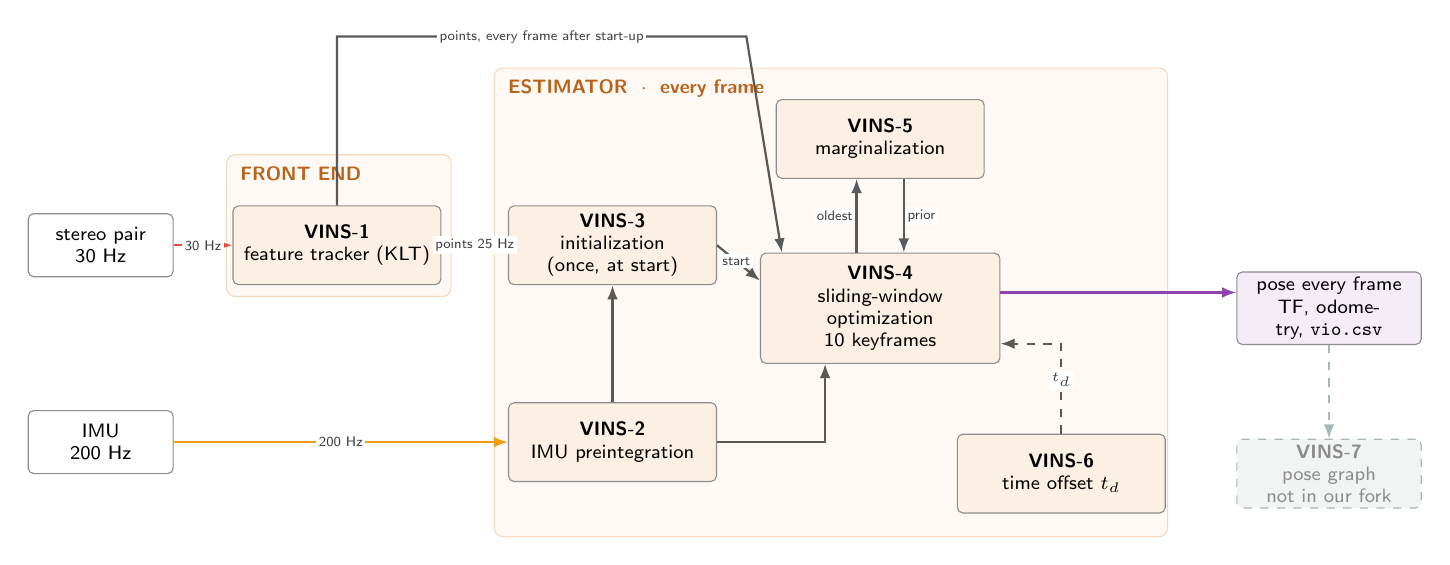
\begin{tikzpicture}[font=\scriptsize,
      cb/.style={box, fill=vinsc!12, text width=25mm, minimum height=10mm},
      bl/.style={font=\scriptsize\bfseries, text=vinsc!80!black, anchor=north west}]
    \fill[vinsc!5, draw=vinsc!30, rounded corners=3pt] (1.6,-0.05) rectangle (4.45,1.75);
    \node[bl] at (1.65,1.72) {FRONT END};
    \fill[vinsc!5, draw=vinsc!30, rounded corners=3pt] (5.0,-3.1) rectangle (13.55,2.85);
    \node[bl] at (5.05,2.82) {ESTIMATOR \;$\cdot$\; every frame};
    \node[box, text width=17mm] (st) at (0,0.6)  {stereo pair\\30 Hz};
    \node[box, text width=17mm] (im) at (0,-1.9) {IMU\\200 Hz};
    \node[cb, VINS1] (v1) at (3.0,0.6)  {\textbf{VINS-1}\\feature tracker (KLT)};
    \node[cb, VINS3] (v3) at (6.5,0.6)  {\textbf{VINS-3}\\initialization\\(once, at start)};
    \node[cb, VINS2] (v2) at (6.5,-1.9) {\textbf{VINS-2}\\IMU preintegration};
    \node[cb, VINS4, text width=29mm, minimum height=14mm] (v4) at (9.9,-0.2)
      {\textbf{VINS-4}\\sliding-window optimization\\10 keyframes};
    \node[cb, VINS5] (v5) at (9.9,1.95) {\textbf{VINS-5}\\marginalization};
    \node[cb, VINS6] (v6) at (12.2,-2.3) {\textbf{VINS-6}\\time offset $t_d$};
    \node[box, text width=22mm, fill=dpose!10] (out) at (15.6,-0.2)
      {pose every frame\\TF, odometry, \repo{vio.csv}};
    \node[box, off, text width=22mm, VINS7] (v7) at (15.6,-2.3) {\textbf{VINS-7}\\pose graph\\not in our fork};
    \draw[arr, dimg] (st) -- node[rate]{30 Hz} (v1);
    \draw[arr, dimu] (im) -- node[rate]{200 Hz} (v2);
    \draw[arr] (v1) -- node[rate]{points 25 Hz} (v3);
    \draw[arr] (v2) -- (v3);
    \draw[arr] (v3.east) -- node[rate, pos=0.45]{start} ($(v4.west)+(0,0.35)$);
    \draw[arr] (v2.east) -| ($(v4.south)+(-0.7,0)$);
    \draw[arr] (v1.north) |- (8.2,3.25) -- ($(v4.north)+(-1.25,0)$);
    \node[rate] at (5.6,3.25) {points, every frame after start-up};
    \draw[arr] ($(v4.north)+(-0.3,0)$) -- node[rate, left]{oldest} ($(v5.south)+(-0.3,0)$);
    \draw[arr] ($(v5.south)+(0.3,0)$) -- node[rate, right]{prior} ($(v4.north)+(0.3,0)$);
    \draw[darr] (v6.north) |- node[rate, pos=0.3]{$t_d$} ($(v4.east)+(0,-0.45)$);
    \draw[arr, dpose] ($(v4.east)+(0,0.2)$) -- ($(out.west)+(0,0.2)$);
    \draw[darr, offc] (out) -- (v7);
  \end{tikzpicture}
%% page 4: RTAB-Map
  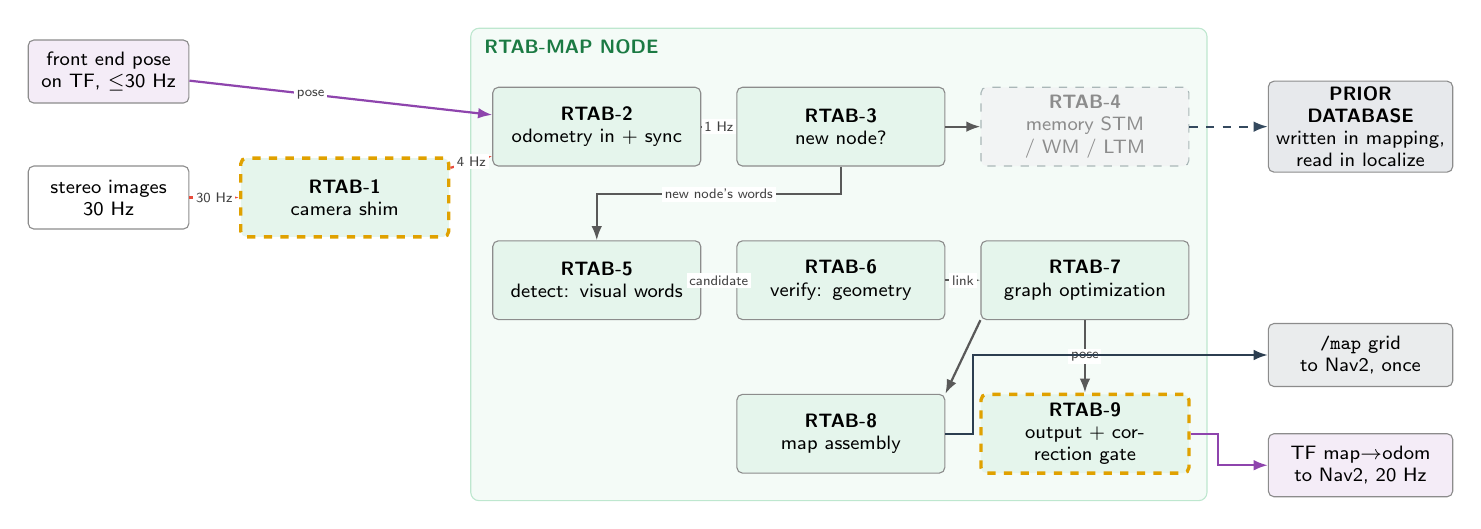
\begin{tikzpicture}[font=\scriptsize,
      cb/.style={box, fill=rtabc!12, text width=25mm, minimum height=10mm},
      bl/.style={font=\scriptsize\bfseries, text=rtabc!70!black, anchor=north west}]
    \fill[rtabc!5, draw=rtabc!30, rounded corners=3pt] (4.6,-4.45) rectangle (13.95,1.55);
    \node[bl] at (4.65,1.52) {RTAB-MAP NODE};
    \node[box, text width=19mm, fill=dpose!10] (fe) at (0,1.0) {front end pose\\on TF, $\le$30 Hz};
    \node[box, text width=19mm] (cams) at (0,-0.6) {stereo images\\30 Hz};
    \node[cb, ours, RTAB1] (r1) at (3.0,-0.6) {\textbf{RTAB-1}\\camera shim};
    \node[cb, RTAB2] (r2) at (6.2,0.3)  {\textbf{RTAB-2}\\odometry in + sync};
    \node[cb, RTAB3] (r3) at (9.3,0.3)  {\textbf{RTAB-3}\\new node?};
    \node[cb, off, RTAB4] (r4) at (12.4,0.3) {\textbf{RTAB-4}\\memory STM / WM / LTM};
    \node[cb, RTAB5] (r5) at (6.2,-1.65) {\textbf{RTAB-5}\\detect: visual words};
    \node[cb, RTAB6] (r6) at (9.3,-1.65) {\textbf{RTAB-6}\\verify: geometry};
    \node[cb, RTAB7] (r7) at (12.4,-1.65) {\textbf{RTAB-7}\\graph optimization};
    \node[cb, RTAB8] (r8) at (9.3,-3.6) {\textbf{RTAB-8}\\map assembly};
    \node[cb, ours, RTAB9] (r9) at (12.4,-3.6) {\textbf{RTAB-9}\\output + correction gate};
    \node[box, text width=22mm, fill=mapcol!12] (db) at (15.9,0.3) {\textbf{PRIOR DATABASE}\\written in mapping,\\read in localize};
    \node[box, text width=22mm, fill=dmap!10] (om) at (15.9,-2.6) {\texttt{/map} grid\\to Nav2, once};
    \node[box, text width=22mm, fill=dpose!10] (ot) at (15.9,-4.0) {TF map$\rightarrow$odom\\to Nav2, 20 Hz};
    \draw[arr, dpose] (fe) -- node[rate, pos=0.4]{pose} (r2);
    \draw[arr, dimg] (cams) -- node[rate]{30 Hz} (r1);
    \draw[arr, dimg] (r1) -- node[rate]{4 Hz} (r2);
    \draw[arr] (r2) -- node[rate]{1 Hz} (r3);
    \draw[arr] (r3) -- (r4);
    \draw[arr] (r3.south) -- ++(0,-0.35) -| node[rate, pos=0.25]{new node's words} (r5.north);
    \draw[arr] (r5) -- node[rate]{candidate} (r6);
    \draw[arr] (r6) -- node[rate]{link} (r7);
    \draw[arr] (r7.south) -- node[rate]{pose} (r9.north);
    \draw[arr] (r7.south west) -- (r8.north east);
    \draw[darr, mapcol] (r4.east) -- (db.west);
    \draw[arr, dmap] (r8.east) -- ++(0.35,0) |- (om.west);
    \draw[arr, dpose] (r9.east) -- ++(0.35,0) |- (ot.west);
  \end{tikzpicture}
\end{document}
